\documentclass[10pt,twocolumn,letterpaper]{article}

\usepackage{cvpr}
\usepackage{times}
\usepackage{epsfig}
\usepackage{graphicx}
\usepackage{amsmath}
\usepackage{amssymb}

\usepackage[breaklinks=true,bookmarks=false]{hyperref}

\cvprfinalcopy % *** Uncomment this line for the final submission

\def\cvprPaperID{****} % *** Enter the CVPR Paper ID here
\def\httilde{\mbox{\tt\raisebox{-.5ex}{\symbol{126}}}}

\setcounter{page}{1}

\begin{document}

%%%%%%%%% TITLE
\title{Wine Quality Prediction}

\author{
Arnav Agrawal\\
IIIT Delhi\\
{\tt\small arnav22097@iiitd.ac.in}
\and
Aryan Singla\\
IIIT Delhi\\
{\tt\small aryan22112@iiitd.ac.in}
\and
Harsh Rajput\\
IIIT Delhi\\
{\tt\small harsh22201@iiitd.ac.in}
\and
Kshitij Gupta\\
IIIT Delhi\\
{\tt\small kshitij22257@iiitd.ac.in}
}

\maketitle

% The purpose of this project is to develop a machine learning pipeline to predict the quality of wines based on physicochemical features. Wine quality prediction is an important problem for producers, as it allows for quality assurance and consistency. In this project, we aim to build a model that can predict wine quality with high accuracy using various regression and classification techniques. Additionally, we plan to explore the usage of machine learning operations (MLOps) techniques to streamline the workflow and manage the model lifecycle.

%%%%%%%%% ABSTRACT
\begin{abstract}
We build a learning system for multi-class classification problems that consists of standard tabular data pre-processing methods, various general training scripts for classical Machine Learning methods as well as Deep and Shallow Learning architectures along with options for regularization techniques and normalization. This framework allows visualisation and comparison of evaluation graphs for the purpose of hyper-parameter tuning using the WandB software. The goal is to create a simple and interactive interface for processing data, training models, evaluating, inferencing, and tuning hyperparameters. Code for this pipeline is available on https://github.com/Boltnav/Wine-Quality-Prediction with setup instructions provided.
\end{abstract}

\section{Introduction}
Wine quality assessment is an important factor maintaining consistency and value in the wine industry. Accurate prediction of wine quality, based on physicochemical features, helps wine producers ensure that their product meets certain standards. Traditional methods of wine quality assessment are time-consuming and subjective. This project develops an \textit{end-to-end automated machine learning pipeline} to predict wine quality based on features such as acidity, alcohol content, and residual sugar.

Wine quality is rated on a discrete scale from 3 to 8, making this an ordinal classification problem. The objective is to use various machine learning and deep learning techniques, specifically classification models, to predict these scores. Additionally, this project explores MLOps practices for managing the model lifecycle.

\section{Related Works}

Previous studies on wine quality prediction have applied a variety of machine learning models \cite{dahal2021}. Methods like Ridge Regression, Support Vector Machine, Gradient Boosting Regressor, and multi-layer Artificial Neural Network, with non-linear models such as Random Forest and Gradient Boosting consistently outperforming linear models. These ensemble methods capture complex feature interactions and non-linearities, which are essential for improving prediction accuracy. The analysis
showed that Gradient Boosting Regressor surpassed all other models’ performance.

Also, \cite{jain2023} utilized Random Forests and Extreme Gradient Boosting. Using these two ML approaches, they chose the top three features from a total of eleven features on the basis of Dimensionality Reduction, and analysis was performed on the
remaining features. They displayed several visualizations that showed that only these three were relevant to the target class, and that they could reduce the feature space and not lose out on many relevant vectors. They employed the XGBoost model and Random Forests to demonstrate this feature importance based selection.

\section{Dataset details}

\subsection{Dataset Acquisition}
The Wine Quality dataset was sourced from the \href{https://www.kaggle.com/datasets/yasserh/wine-quality-datasety}{Kaggle Machine Learning Repository}. It contains physicochemical features of red and white wine samples, with quality scores ranging from 3 to 8. The dataset contains 12 attributes related to the wine’s composition, including fixed acidity, volatile acidity, residual sugar, chlorides, and alcohol content.

\subsection{Data Preprocessing}
Initial exploration revealed no missing values in the dataset. The features were standardized using \textbf{StandardScaler} to ensure equal contribution to the models. Since the dataset showed a class imbalance, where most wines were rated between 5 and 6, we applied \textbf{SMOTE} (Synthetic Minority Over-sampling Technique) to generate synthetic samples for the minority classes and balance the dataset.

\begin{figure}[h]
    \centering
    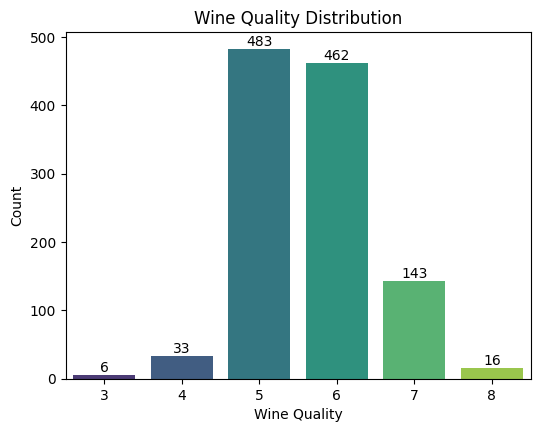
\includegraphics[width=1\linewidth]{cvpr2019AuthorKit/images/output1.png}
    \caption{Class imbalance in the dataset.}
\end{figure}

% \begin{figure}[h]
%     \centering
%     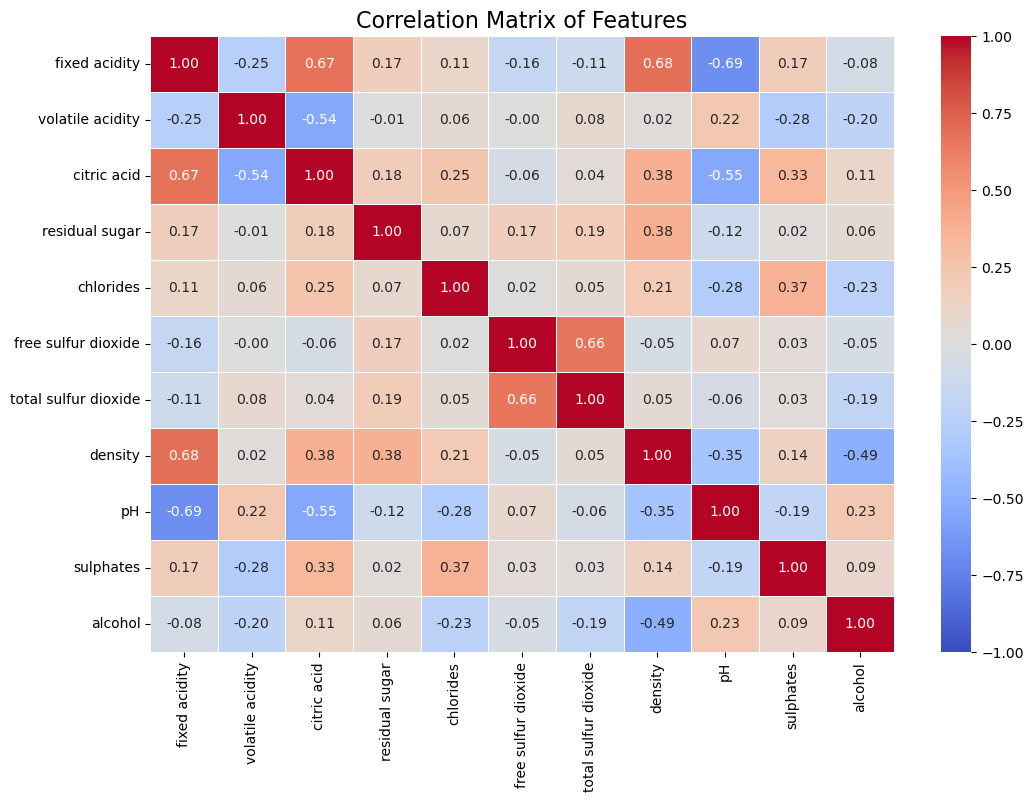
\includegraphics[width=1\linewidth]{cvpr2019AuthorKit/images/output2.png}
%     \caption{Correlation matrix of the dataset.}
% \end{figure}

\section{Methodology and Model Details}

We compare how quickly models converge by analyzing training loss over epochs:

\subsection{Deep Learning Models}

We started of by using the original dataset on a shallow Neural Network involving only a singular hidden layer of  64 neurons. Initially, this proved to be a naive attempt, as we saw observed 99\% train accuracy but only 55\% validation and 20\% test accuracies. This was clear evidence of overfitting, as the validation accuracy didn't increase and the validation loss didn't decrease for atleast a few 100 epochs. We performed early stopping for the same, and the model ran for about 20 epochs before converging with about 60\% validation and test accuracies. 

This was clear evidence of class imbalance and a full roadblock  on the idea of using the unedited original data. Hence, we performed further experiments on the dataset we obtained from applying the Synthetic Minority Over-Sampling Technique. 

\begin{itemize}
    \item \textbf{Shallow Neural Network}: Beginning with a simple single-hidden layer architecture, this gave us 85\% accuracy upon performing on the test, with train 
    \begin{figure}
        \centering
        \includegraphics[width=0.5\linewidth]{NN1.png}
        \caption{Single Hidden Layer Architecture}
        \label{Shallow NN}
    \end{figure}
    \item 


\end{itemize}

To do better, we used the tool WandB.ai. We performed 

\subsection{Models Used}
We implemented both regression and classification models to predict wine quality. However, wine quality prediction is inherently a classification problem, as the target variable is a discrete quality score (3 to 8). Below is a summary of the models used:

\begin{itemize}
    \item \textbf{Linear Regression}: Predicts continuous approximations of wine quality scores. This method is suboptimal because it predicts continuous values that must be rounded, introducing errors.
    
    \item \textbf{Ridge and Lasso Regression}: Add regularization to avoid overfitting, but face the same limitations as Linear Regression for classification tasks.
    
    \item \textbf{Logistic Regression}: A linear classifier that models the probability of each class but struggles with non-linear relationships.
    
    \item \textbf{Random Forest}: An ensemble method that builds multiple decision trees to capture non-linear relationships in the data. Performs well due to its ability to model complex feature interactions.
    
    \item \textbf{Gradient Boosting}: Builds decision trees sequentially, correcting errors from the previous model. Provides high accuracy, comparable to Random Forest.
\end{itemize}

\begin{figure}[h]
    \centering
    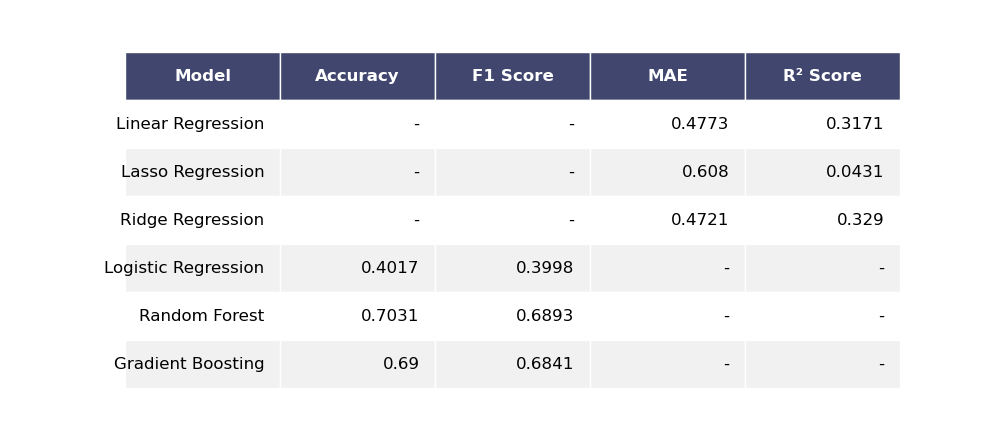
\includegraphics[width=1\linewidth]{cvpr2019AuthorKit/images/output5.png}
    \caption{Comparison of model performance.}
\end{figure}

\subsection{Regression Models on Classification Problems}
Regression models like \textbf{Linear Regression}, \textbf{Ridge Regression}, and \textbf{Lasso Regression} were applied, but their continuous predictions required rounding, leading to poor classification results.

\textbf{Why Regression Fails:}
\begin{itemize}
    \item \textbf{Continuous Output}: Regression models predict continuous values that must be rounded, introducing errors.
    \item \textbf{Lack of Decision Boundaries}: Regression models do not define clear boundaries between classes, which is crucial for classification tasks.
    \item \textbf{Linear Assumptions}: These models assume linear relationships between features and target, which is not the case with wine quality data.
\end{itemize}

\begin{figure}[h]
    \centering
    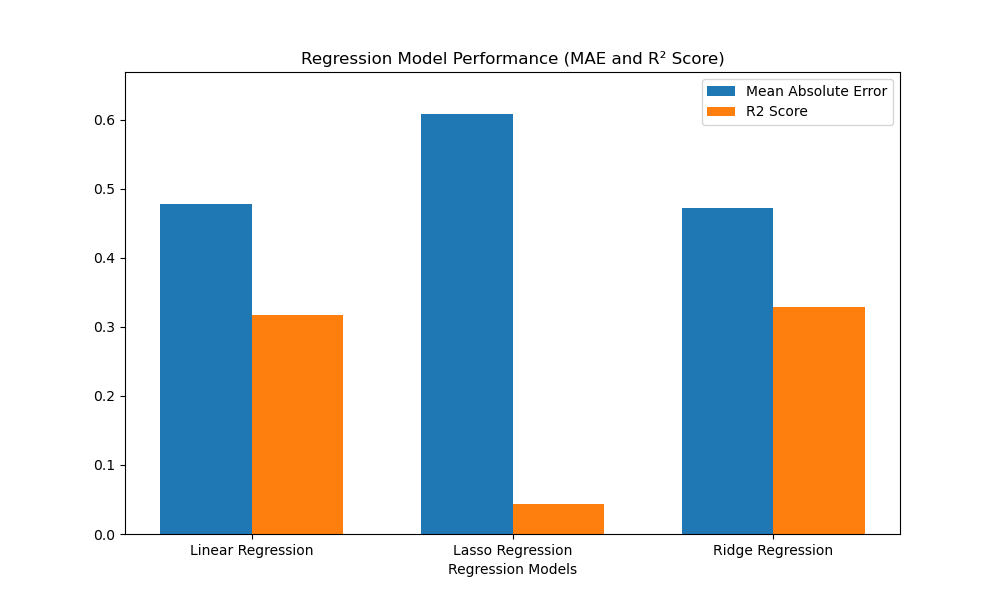
\includegraphics[width=1\linewidth]{cvpr2019AuthorKit/images/output4.png}
    \caption{Regression models perform poorly on classification tasks.}
\end{figure}

\subsection{Classification Model Results}
Classification models performed significantly better, with \textbf{Random Forest} and \textbf{Gradient Boosting} outperforming logistic regression due to their ability to capture non-linear patterns.

\textbf{Classification Model Performance}:
\begin{itemize}
    \item \textbf{Logistic Regression}: Accuracy = 40.17\%, F1 Score = 0.3998.
    \item \textbf{Random Forest}: Accuracy = 70.31\%, F1 Score = 0.6893.
    \item \textbf{Gradient Boosting}: Accuracy = 69.00\%, F1 Score = 0.6841.
\end{itemize}

\begin{figure}[h]
    \centering
    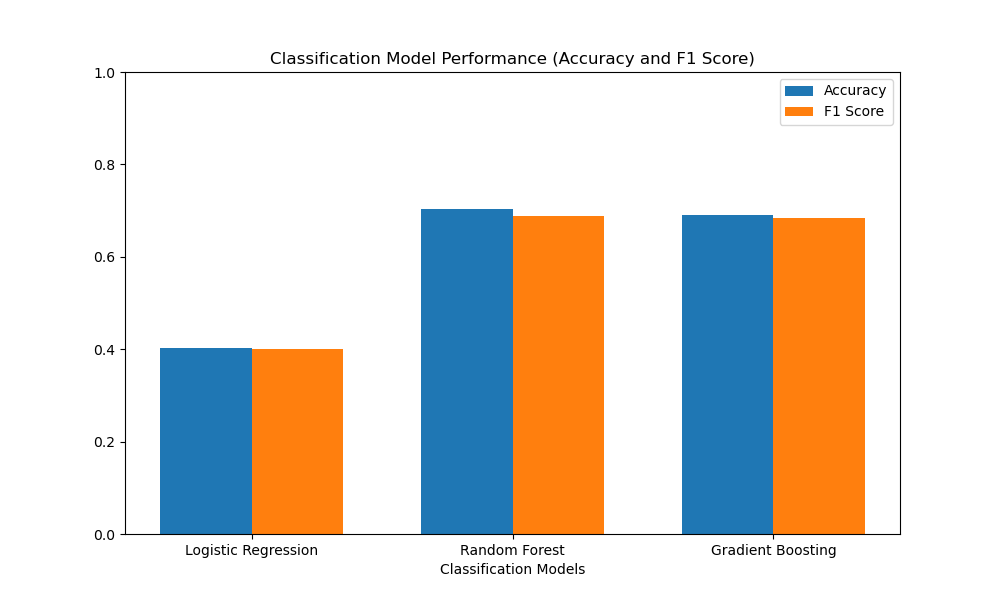
\includegraphics[width=1\linewidth]{cvpr2019AuthorKit/images/output3.png}
    \caption{Performance of classification models.}
\end{figure}

\subsection{MLOps Pipeline}
We implemented an MLOps pipeline to manage the model lifecycle, including data ingestion, preprocessing, model training, and evaluation. Experiment tracking was handled through version control, ensuring reproducibility. In future work, we aim to containerize the models using Docker for easier deployment and scaling.

\section{Results and Analysis}

\subsection{Regression Models}
Regression models struggled with predicting discrete quality scores. After rounding, the performance was significantly worse compared to classification models.
\begin{itemize}
    \item \textbf{Linear Regression}: $R^2$ = 0.3171, Mean Squared Error = 0.4773.
    \item \textbf{Lasso Regression}: $R^2$ = 0.0431, Mean Squared Error = 0.6080.
    \item \textbf{Ridge Regression}: $R^2$ = 0.3290, Mean Squared Error = 0.4721.
\end{itemize}

\subsection{Classification Models}
\begin{itemize}
    \item \textbf{Logistic Regression}: Accuracy = 40.17\%, F1 Score = 0.3998.
    \item \textbf{Random Forest}: Accuracy = 70.31\%, F1 Score = 0.6893.
    \item \textbf{Gradient Boosting}: Accuracy = 69.00\%, F1 Score = 0.6841.
\end{itemize}

\section{Conclusion}
In this project, we explored both regression and classification models for predicting wine quality. Classification models, particularly ensemble methods like Random Forest and Gradient Boosting, performed significantly better than regression models. This is because the classification models are better suited to handle non-linear relationships between features and discrete target classes, which is essential for predicting wine quality effectively. 

We successfully implemented a basic MLOps pipeline to manage the model lifecycle, covering data ingestion, preprocessing, model training, and evaluation. The initial experiment tracking was also integrated with version control, ensuring reproducibility and experiment transparency.

\subsection{Future Work}
In the future, we aim to implement a full end-to-end MLOps pipeline to automate and streamline the machine learning workflow. This includes the following:

\begin{itemize}
    \item \textbf{Hyperparameter Tuning}: Applying advanced techniques like grid search and randomized search to optimize model hyperparameters for the best performance.
    \item \textbf{Model Deployment}: Containerizing the models using Docker and deploying them to cloud environments (such as AWS, GCP, or Azure) for scalability and accessibility.
    \item \textbf{Continuous Integration/Continuous Deployment (CI/CD)}: Setting up automated pipelines for retraining, testing, and deploying models based on new data or performance degradation, ensuring that the model stays up-to-date and efficient.
    \item \textbf{Model Monitoring}: Implementing real-time model monitoring to track the performance of models in production, enabling quick response to performance drops or data drift.
    \item \textbf{Data Versioning and Experiment Tracking}: Using tools like DVC (Data Version Control) and MLflow to maintain organized version control for datasets and experiments, further enhancing reproducibility and collaboration.
\end{itemize}

By building a fully automated and scalable MLOps framework, we can continuously improve the model's accuracy and reliability while minimizing manual intervention and reducing time-to-deployment.

\subsection{Contribution}
\begin{itemize}
    \item \textbf {Arnav Agrawal:} EDA, Model implementation 
    \item \textbf {Aryan Singla:} EDA, Inference 
    \item \textbf {Harsh Rajput:} Preprocessing, Model implementation
    \item \textbf {Kshitij Gupta:} Preprocessing, Inference 
\end{itemize}

\section{References}
{\small
\bibliographystyle{ieee_fullname}
\bibliography{references}
}

\end{document}
